% ------------------------------------------------------------------
\documentclass[12 pt]{article} % A4 paper set by geometry package below
\pagenumbering{arabic}
\setlength{\parindent}{10 mm}
\setlength{\parskip}{12 pt}

% Nimbus Sans font should be reasonably legible
\usepackage{helvet}
\renewcommand{\familydefault}{\sfdefault}
\usepackage[T1]{fontenc}  % Without this \textsterling produces $

% Section header spacing
\usepackage{titlesec}
\titlespacing\section{0pt}{12pt plus 4pt minus 2pt}{0pt plus 2pt minus 2pt}
\titlespacing\subsection{0pt}{12pt plus 4pt minus 2pt}{0pt plus 2pt minus 2pt}
\titlespacing\subsubsection{0pt}{12pt plus 4pt minus 2pt}{0pt plus 2pt minus 2pt}

\usepackage{amsmath}
\usepackage{amssymb}
\usepackage{graphicx}
\usepackage{verbatim}    % For comment
\usepackage[paper=a4paper, marginparwidth=0 cm, marginparsep=0 cm, margin=2.5 cm, includemp]{geometry}
\usepackage[pdftex, pdfstartview={FitH}, pdfnewwindow=true, colorlinks=true, citecolor=blue, filecolor=blue, linkcolor=blue, urlcolor=blue, pdfpagemode=UseNone]{hyperref}

% Put module code and last-modified date in footer
\usepackage{fancyhdr}
\pagestyle{fancy}
\fancyhf{}
\renewcommand{\headrulewidth}{0pt}
\cfoot{{\small \thisunit}\hfill \thepage\hfill {\small \moddate}}

% Hopefully address Canvas complaints about pdf tagging
%\usepackage[tagged]{accessibility}
\hypersetup {
  pdfauthor={David Schaich},
  pdftitle={StatMech Tutorial},
}
% ------------------------------------------------------------------



% ------------------------------------------------------------------
\begin{document}
\newcommand{\thisunit}{MATH327 Tutorial (Cycle)}
\newcommand{\moddate}{Last modified 12 Mar.~2025}
\begin{center}
  {\Large \textbf{MATH327: StatMech and Thermo, Spring 2025}} \\[12 pt]
  {\Large \textbf{Tutorial exercises \ --- \ Otto cycle}} \\[24 pt]
\end{center}

These exercises will be introduced in our 13 March tutorial, and you'll have the week until our next tutorial on 20 March to work on them.
They expand our analyses of thermodynamic cycles to a more realistic example illustrated by the PV~diagram below.
This is known as the `Otto cycle', and describes an idealized petrol engine.

\vspace{-12 pt}
\begin{center}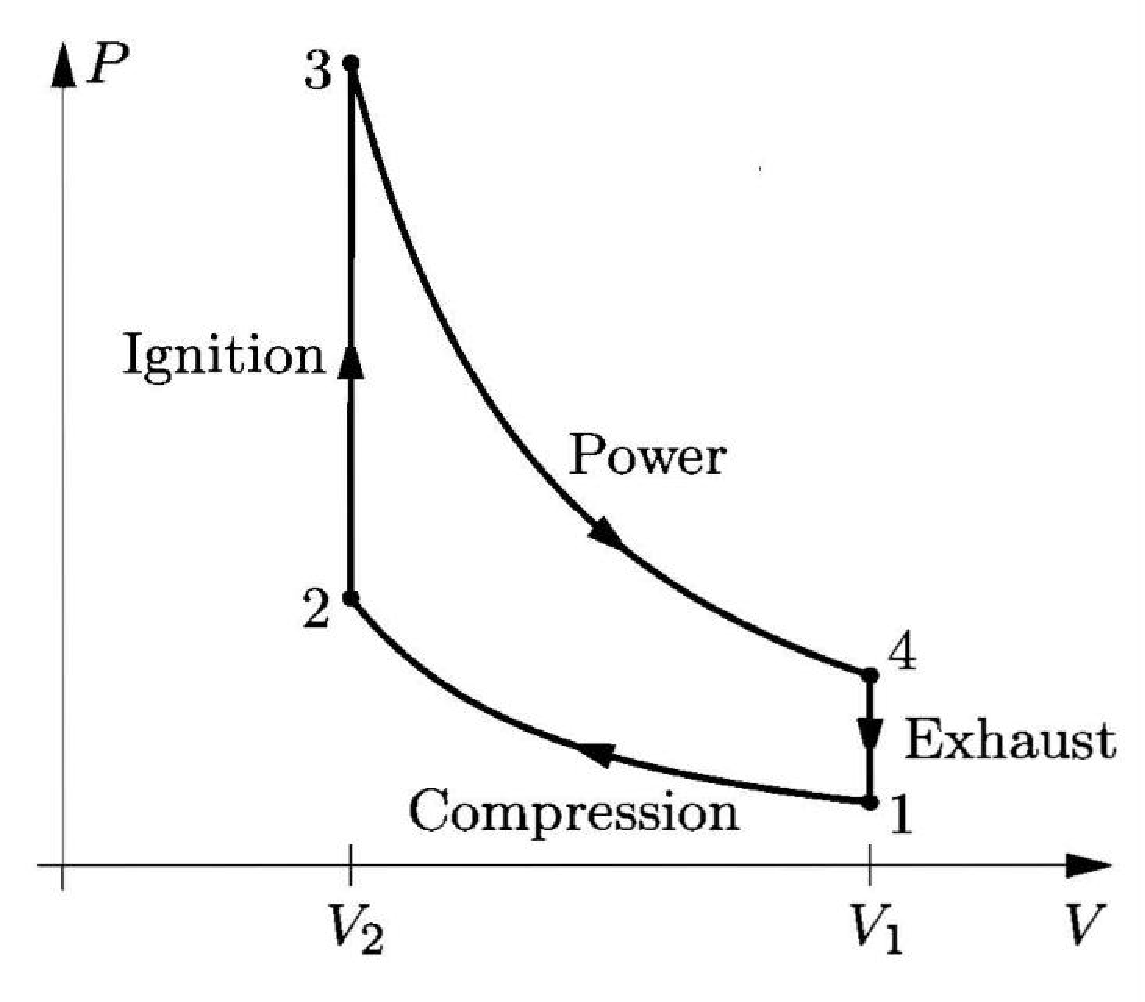
\includegraphics[width=0.6\textwidth]{figs/Otto.pdf}\end{center}
\vspace{-12 pt}

Start by determining the work and heat associated with each of the four processes connecting points $1 \to 2 \to 3 \to 4 \to 1$: \\[-30 pt]
\begin{itemize}
  \item Fast (adiabatic) compression increases the pressure of the gas (a mixture of air and vaporized petrol), until a spark ignites it.
  \item This ignition introduces lots of heat almost instantaneously, while the volume is fixed at $V_2$.
        Even though the gas itself is burning, we can interpret this heat as coming from energy exchange with a hot thermal reservoir.
  \item In the `power' stage the gas adiabatically expands back to volume $V_1 > V_2$. % Note no slow isothermal stages...
  \item Finally, heat is expelled at fixed volume $V_1$ by swapping the hot exhaust for an equal amount of cooler, fresh gas ready to be burned.
\end{itemize}

Putting these ingredients together, what is the efficiency $\eta$ of the Otto cycle?
You should find that $\eta$ is a function of the \textbf{compression ratio}
\begin{equation*}
  r \equiv \frac{V_1}{V_2} > 1.
\end{equation*}
How does the efficiency of the Otto cycle compare to that of the Carnot cycle?
How should $V_1$ and $V_2$ be chosen to maximize the efficiency?

\textbf{Hint:} Given the labels in the PV~diagram above, $T_1$ is the low temperature of the cold reservoir while $T_3$ is the high temperature of the hot reservoir.
The corresponding Carnot cycle efficiency is therefore $\eta_C = 1 - \frac{T_1}{T_3}$, and the comparison is easiest if the Otto cycle efficiency is expressed in terms of temperatures rather than volumes.

\end{document}
% ------------------------------------------------------------------
